\documentclass[12pt]{article}
\usepackage{geometry} % Pour passer au format A4
\geometry{hmargin=1cm, vmargin=1cm} % 

% Page et encodage
\usepackage[T1]{fontenc} % Use 8-bit encoding that has 256 glyphs
\usepackage[english,french]{babel} % Français et anglais
\usepackage[utf8]{inputenc} 

\usepackage{lmodern}
\setlength\parindent{0pt}

% Graphiques
\usepackage{graphicx,float,grffile}

% Maths et divers
\usepackage{amsmath,amsfonts,amssymb,amsthm,verbatim}
\usepackage{multicol,enumitem,url,eurosym,gensymb}

% Sections
\usepackage{sectsty} % Allows customizing section commands
\allsectionsfont{\centering \normalfont\scshape}

% Tête et pied de page

\usepackage{fancyhdr} 
\pagestyle{fancyplain} 

\fancyhead{} % No page header
\fancyfoot{}

\renewcommand{\headrulewidth}{0pt} % Remove header underlines
\renewcommand{\footrulewidth}{0pt} % Remove footer underlines

\newcommand{\horrule}[1]{\rule{\linewidth}{#1}} % Create horizontal rule command with 1 argument of height

%----------------------------------------------------------------------------------------
%	Début du document
%----------------------------------------------------------------------------------------

\begin{document}

%----------------------------------------------------------------------------------------
% RE-DEFINITION
%----------------------------------------------------------------------------------------
% MATHS
%-----------

\newtheorem{Definition}{Définition}
\newtheorem{Theorem}{Théorème}
\newtheorem{Proposition}{Propriété}

% MATHS
%-----------
\renewcommand{\labelitemi}{$\bullet$}
\renewcommand{\labelitemii}{$\circ$}
%----------------------------------------------------------------------------------------
%	Titre
%----------------------------------------------------------------------------------------

\setlength{\columnseprule}{1pt}

\horrule{2px}
\section*{Chapitre 1 - Théorème de Pythagore}
\horrule{2px}

\begin{enumerate}
	\item[1.] Connaissances
	      \begin{itemize}
		      \item Opération Carré : $x^2$
		      \item Opération Racine carré : $\sqrt{x}$
		      \item Connaitre le Théorème
	      \end{itemize}
	\item[2.] Compétences
	      \begin{itemize}
		      \item Savoir quand utiliser le théorème de Pythagore.
		      \item Savoir calculer une longueur à l'aide du théorème de Pythagore.
	      \end{itemize}
\end{enumerate}

\section*{1 - Le carré}

\begin{Definition}
	Un carré est une figure géométrique qui possède 4 côtés de même longueur et 4 angles droits.
\end{Definition}

Soit un carré de côté $c$.
\begin{itemize}
	\item Périmètre : $4 \times c = 4c$
	\item Aire : $c \times c = c^2$
\end{itemize}

\begin{multicols}{2}

	\subsection*{L'opération carré}

	\textbf{L'opération : $x^2$ permet de trouver l'aire d'un carré à partir de son côté.} \\
	\textbf{On multiplie un nombre par ce même nombre.}

	\underline{Liste des premiers carrés :}

	\begin{itemize}
		\item $1^2 = 1 \times 1 = 1$
		\item $2^2 = 2 \times 2 = 4$
		\item $3^2 = 3 \times 3 = 9$
		\item $4^2 = 4 \times 4 = 16$
		\item $5^2 = 5 \times 5 = 25$
		\item $6^2 = 6 \times 6 = 36$
		\item $7^2 = 7 \times 7 = 49$
		\item $8^2 = 8 \times 8 = 64$
		\item $9^2 = 9 \times 9 = 81$
		\item $10^2 = 10 \times 10 = 100$
		\item $11^2 = 11 \times 11 = 121$
		\item $12^2 = 12 \times 12 = 144$
	\end{itemize}

	\subsection*{L'opération racine carré}

	\textbf{L'opération : $\sqrt{x}$ permet de trouver le côté d'un carré à partir de son aire.}\\
	\textit{Sans calculatrice, cette opération peut se révéler compliquée.}

	\underline{Liste des premières racines : }

	\begin{itemize}
		\item $\sqrt{1} = 1$
		\item $\sqrt{4} = 2$
		\item $\sqrt{9} = 3$
		\item $\sqrt{16} = 4$
		\item $\sqrt{25} = 5$
		\item $\sqrt{36} = 6$
		\item $\sqrt{49} = 7$
		\item $\sqrt{64} = 8$
		\item $\sqrt{81} = 9$
		\item $\sqrt{100} = 10$
		\item $\sqrt{121} = 11$
		\item $\sqrt{144} = 12$
	\end{itemize}
\end{multicols}

\newpage
\section*{2 - Modéliser}

\textit{Quand utiliser le théorème de Pythagore ?}\\

On utilise \textbf{le théorème de Pythagore} lorsqu'on cherche à \underline{\textbf{calculer la longueur d'un côté}} dans un \textbf{triangle rectangle} en connaissant \textbf{deux côtés}.



\section*{3 - Théorèmes}

Il existe beaucoup de démonstrations du théorème.

\begin{itemize}
	\item \url{https://www.geogebra.org/m/PujhpZtM}
	\item \url{https://www.youtube.com/watch?v=CAkMUdeB06o}
	\item \url{https://www.youtube.com/watch?v=o1L86rJWkBc&t=61s}
	\item Euclide - Les éléments - Livre 1 - p48.
\end{itemize}


\begin{Definition}
	Dans un triangle rectangle, le plus grand côté s'appelle \textbf{l'hypoténuse}. Il est opposé à l'angle droit.
\end{Definition}



\begin{Theorem}{Énoncé géométrique}\\
	Dans un triangle rectangle, l'aire du carré issue de l'hypoténuse est égale à la somme des aires des carrés issues des deux autres côtés.
\end{Theorem}

\begin{Theorem}{Énoncé général}\\
	Dans un triangle rectangle, le carré de l'hypténuse est égale à la somme des carrés des deux autres côtés.
\end{Theorem}


\begin{Theorem}{Énoncé exercice}\\

	\begin{figure}[H]
		\centering
		\includegraphics[width=0.3\linewidth]{4x1-pythagore/sources/thm-exo.pdf}
	\end{figure}
	
	\begin{enumerate}
		\item[1.] Dans le triangle ABC rectangle en A.
		\item[2.] D'après le théorème de Pythagore.
		\item[3.] $BC^2 = AB^2 + AC^2$
	\end{enumerate}
\end{Theorem}

\newpage
\section*{4 - Calcul du troisième côté}

Il faut être prudent quand on utilise le théorème de Pythagore car il y a une différence si on cherche un hypoténuse ou un petit côté.

\begin{multicols}{2}

	\subsection*{Recherche d'un hypoténuse}

	\begin{figure}[H]
		\centering
		\includegraphics[width=0.5\linewidth]{4x1-pythagore/sources/re-h.pdf}
	\end{figure}

	Dans le triangle MNO rectangle en O.\\
	D'après le théorème de Pythagore.
	\begin{eqnarray*}
		MN^2 &=& MO^2 + NO^2 \\
		MN^2 &=& 20^2 + 32^2 \\
		MN   &=& \sqrt{20^2 + 32^2} \\
		MN   &\approx& 37.7
	\end{eqnarray*}

	La longueur MN mesure environ 27.7cm.


\end{multicols}
\begin{multicols}{2}
	\subsection*{Recherche d'un petit côté}

	\begin{figure}[H]
		\centering
		\includegraphics[width=0.5\linewidth]{4x1-pythagore/sources/re-c.pdf}
	\end{figure}

	Dans le triangle MNO rectangle en O.\\
	D'après le théorème de Pythagore.
	\begin{eqnarray*}
		MN^2 &=& MO^2 + NO^2 \\
		40^2 &=& MO^2 - 12^2 \\
		MO^2 &=& 40^2 - 12^2 \\
		MO   &=& \sqrt{40^2 - 12^2} \\
		MO   &=& 38
	\end{eqnarray*}

	La longueur MO mesure 38cm.

\end{multicols}
\subsection*{Problème}

\textbf{Énoncé} J'ai oublié mes clés pour rentrer chez moi. La fenêtre du premier étage est ouverte.
Le bas de la fenêtre se trouve à 4m du sol. Un voisin me prête une échelle de 4.5m de long.
Pour monter à l'échelle sans tomber, je suis obligé de poser les pieds de l'échelle à au moins 1.5 m du pied du mur.\\
\textbf{Pourrai-je atteindre le bas de ma fenêtre ?}

\begin{multicols}{2}

	\textbf{Je représente la situation}

	\begin{figure}[H]
		\centering
		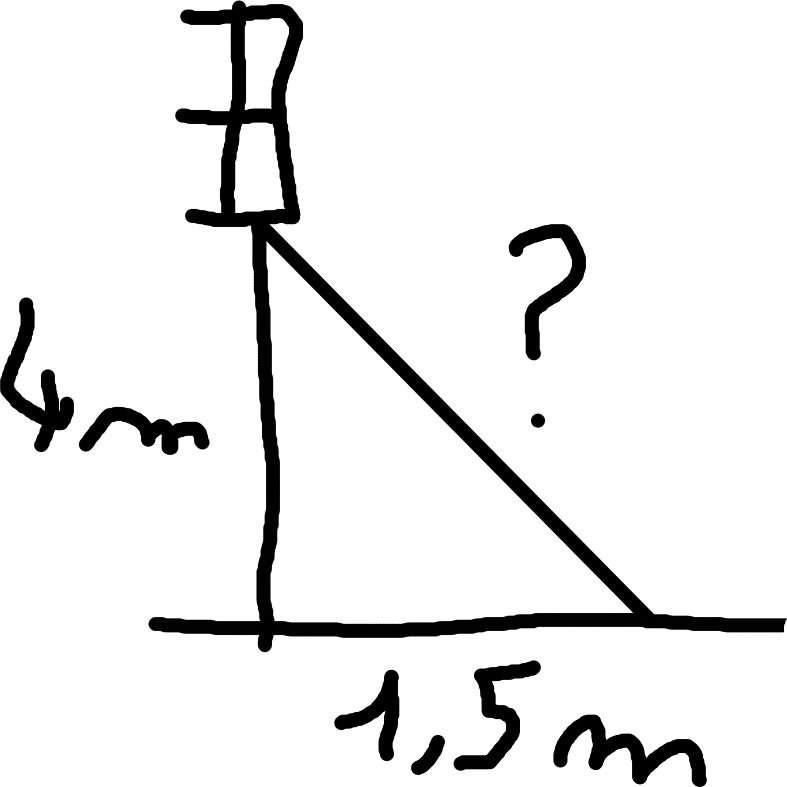
\includegraphics[width=0.5\linewidth]{4x1-pythagore/sources/probleme.jpg}
	\end{figure}

	\textit{J'ai un triangle rectangle, j'ai deux longueurs, je cherche la troisième pour la comparer avec l'échelle.}\\
	\textbf{Je peux utiliser le théorème de Pythagore.}
	\vspace{1cm}
	\underline{\textbf{Rédiger}}\\
	Le triangle est rectangle.\\
	On appelle $x$ la longueur cherchée.\\
	D'après le théorème de Pythagore.

	\begin{eqnarray*}
		x^2 &=& 4^2 + 1.5^2 \\
		x   &=& \sqrt{4^2 + 1.5^2} \\
		x   &\approx& 4.27
	\end{eqnarray*}

	Comme 4.27m < 4.5m, \textit{(la longueur x entre la fenêtre et le sol est plus petite que l'échelle.)}\\
	\textbf{L'echelle est suffisament grande.}
\end{multicols}
\end{document}
